\documentclass[%handout,
	sans,
	12pt,
	%slidescentered,% center text on slide
	%draft,			% compile as draft version
	%notes,			% include nodes in slides
	%compress		% compress navigation bar
]{beamer}

\beamertemplatenavigationsymbolsempty

\usetheme{default}
\usecolortheme{orchid}
\setbeamertemplate{frametitle}
{
    \vspace*{1.5em}\insertframetitle\vspace*{-1.5em}
}
\setbeamertemplate{footline}[frame number]

\usepackage[T1]{fontenc}
\usepackage[utf8x]{inputenc}

\usepackage{mathpazo}
\usepackage[british]{babel}
\usepackage{csquotes}

\newcommand{\high}[1]{{\usebeamercolor[fg]{structure} #1}}
\newcommand{\bad}[1]{\textcolor{red}{#1}}
\newcommand{\gray}[1]{\textcolor{darkgray}{#1}}
\newcommand{\black}[1]{\textcolor{black}{#1}}

\usepackage{amsmath,amssymb}
\usepackage{upgreek}
\usepackage{booktabs}
\usepackage{hyperref}
\usepackage{graphicx}
\usepackage{colortbl}
\usepackage{url}
\usepackage{setspace}
\usepackage{wrapfig}
\usepackage{tabularx}
\usepackage{xspace}
\usepackage{mathpartir}

\usepackage{tikz}
\usetikzlibrary{trees, positioning}
\usetikzlibrary{shapes.geometric}


\newcommand{\RR}{\mathbb{R}}
\newcommand{\CC}{\mathbb{C}}
\newcommand{\NN}{\mathbb{N}}
\renewcommand{\epsilon}{\varepsilon}
\renewcommand{\phi}{\varphi}
\def\braces#1{[#1]}
\newcommand{\wrt}{w.\,r.\,t.\xspace}
\newcommand{\eg}{e.\,g.\xspace}
\newcommand{\ie}{i.\,e.\xspace}
\DeclareMathOperator\caret{\char`\^}

\newcommand{\hastype}{\,:\,}
\newcommand{\cons}{::}
\newcommand{\corrto}{\overset{\scriptscriptstyle\wedge}{=}}
\newcommand{\listapp}{\mathbin{@}}
\newcommand{\listnil}{[\hskip0.3mm]}
\newcommand{\listnth}{\mathbin{!}}
\newcommand{\expectation}{\text{\upshape E}}

\usepackage{manfnt}
\newenvironment{danger}{\medbreak\noindent\hangindent=2pc\hangafter=-2%
  \clubpenalty=10000%
  \hbox to0pt{\hskip-\hangindent\hskip0.25em\raisebox{-0.25em}[0pt][0pt]{\dbend}\hfill}\small\ignorespaces}%
  {\medbreak\par}
  %\raisebox{-1.05em}[0pt][0pt]{\Huge\hskip.15em \stixdanger}

\newcommand{\etAl}{\textit{et al.}\xspace}

%\definecolor{mybg}{rgb}{0.9,0.9,0.9}
\definecolor{mybg}{rgb}{1,1,1}
\setbeamercolor{background canvas}{bg=mybg}

\title{Field Extensions in \emph{Isabelle/HOL} \vspace*{-0.5em}}
\author{\normalsize Fabian Hellauer}
\institute[]{\footnotesize Technische Universität München}
\date{\footnotesize 6 June 2018 to-do}

\begin{document}

\maketitle

\begin{frame}
\begin{center}

\includegraphics[width=5cm]{isabelle.pdf}
\end{center}
\end{frame}


\newcommand{\pivot}[1]{{\color{red}#1}}
\newcommand{\ltpiv}[1]{{\color{blue}#1}}
\newcommand{\gtpiv}[1]{{\color{olive}#1}}

\begin{frame}{Verification of Mathematics}%in particular widely accepted Mathematics like Linear Algebra
Reasons:
\begin{itemize}
	\item to obtain a basis for more useful results\pause
	%as a computer scientist, I mainly think of algorithms and their correctness
	\item to find mistakes\pause
	\item meta: to prove that verification %of a handfull of pages
	is feasible (when using modern tools)
	%this could be motivation to do more math theories, because it removes the need for experts to get them accepted.
\end{itemize}
\end{frame}

\begin{frame}
\begin{center}
\huge\high{Algebraic Structures in HOL-Algebra}
\end{center}
\end{frame}

\begin{frame}{HOL-Algebra}
\begin{itemize}
	\item record-based \pause%to-do: partial_object_def? how to explain to Prof. K.?
	\item subscripts \pause%to-do: do they even appear in an example?
	\item locale-based \pause%INTEG as example?
	% reasons
	\item explicit carrier sets \pause
	\item enables reasoning about substructures	\pause%this is what we will do
	% HOL-Computational_Algebra uses types --> this is not possible
\end{itemize}
\end{frame}

\begin{frame}{Problems}
\begin{itemize}
\item Bases are sets.
\bad{In the finite case, we often want them as lists. to-do: later? explain non-canonical}
\item Coefficients are functions.
\bad{need to prove membership in the correct function set at \emph{every} step.
	% at least that's what it feels like
	 to-do: details /example?}
\end{itemize}
\begin{itemize}
\item Type $\alpha\ \textit{pmf}$ represents a probability distribution of values of type $\alpha$\pause
\item Isomorphic to the set of functions $f : \alpha\to\mathbb{R}$ with $f(x) \geq 0$ and $\sum_{x :: \alpha} f(x) = 1$\pause
\item Giry monad allows composing PMFs: $\textbf{do}\ \{x\leftarrow A;\ y \leftarrow B\ x;\ \textbf{return}\ (f\ x\ y)\}$
\end{itemize}
\end{frame}

\begin{frame}{Tower rule}
If $M/L$ and $L/K$ are field extensions, then
\[[M : K] = [M : L] \cdot [L : K]\]\pause %ask M.: good idea to use non-HOL notation?
In particular, combining two finite field extensions yields a finite field extension. %(or combining finitely many)
\end{frame}

\begin{frame}{Encoding of $\infty$}
Can we use type \emph{nat} for the degree of field extensions?\pause
\begin{itemize}
	\item The degree is a vector space dimension.\pause%these *can* be zero (iff zvs)
	\item However, it is always $\ge 1$.\pause
	\item Thus, this encoding strips no information:\\%It could be adapted easily to use extended natural numbers
	\textbf{definition} \textit{degree} \textbf{where}\\
	\hskip1em\textit{degree = (if finite then vs.dim else 0)}
\end{itemize}
\end{frame}

\begin{frame}{Contributions}
\begin{itemize}
	\item Vector Spaces\pause
	\item Field Extensions\pause
	\item Misc? to-do
\end{itemize}
\end{frame}

\begin{frame}
Deterministic quicksort with first element as pivot:
\[\text{qs} :: \alpha\ \text{list} \to \alpha\ \text{list}\pause \times \mathbb{N}\]\pause
Quicksort with random pivot:
\[\text{rqs} :: \alpha\ \text{list} \to (\alpha\ \text{list} \times \mathbb{N})\ \text{pmf}\]\pause
Average-case of det.\ quicksort:
\[\text{avqs}\ \textit{xs} = \textbf{do}\ \{\textit{xs'} \leftarrow \text{rperm}\ \textit{xs}\hskip0.2mm;\ \textbf{return}\ (\text{qs}\ \textit{xs'}\hskip0.2mm)\}\]\pause
\vspace*{-1.5em}
\begin{theorem}
\upshape
\begin{itemize}
\item $\expectation[\text{snd}(\text{rqs}\ \text{xs})] = 2(n+1) H_n - 4n \sim 2 n \ln n$\pause
\item $\text{avqs} = \text{rqs}$
\end{itemize}
\end{theorem}
\end{frame}

\begin{frame}
What happens when we insert distinct elements $x_1, \ldots, x_n$ into an empty BST?\\[2em]
\begin{center}
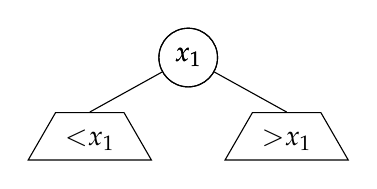
\begin{tikzpicture}[level distance = 1cm, sibling distance=2.5cm]
\action<1>{
\node[shape=circle,draw] {$x_1$};}
\action<2>{
\node[shape=circle,draw] {$x_1$}
  child {node[draw, trapezium, trapezium angle=60, text height=3mm]{${<}x_1$} [child anchor=north]}
  child {node[draw, trapezium, trapezium angle=60, text height=3mm]{${>}x_1$} [child anchor=north]};}
%\action<3->{
%\node[shape=circle,draw] {$x_1$}
%  child {node[shape=circle,draw]{$x_2$}
%         [child anchor=border]
%         child {node[draw, trapezium, trapezium angle=60, text height=3mm]{${<}x_2$} [child anchor=north]}
%         child {node[draw, trapezium, trapezium angle=60, text height=3mm]{${>}x_2$} [child anchor=north]}}
%  child {node[draw, trapezium, trapezium angle=60, text height=3mm]{${>}x_1$} [child anchor=north]};}
\end{tikzpicture}\hspace*{2em}
\end{center}
\end{frame}

\begin{frame}
$\small\text{mk\_bst}\ \listnil = \hskip2.64cm \bullet$\\[1em]\pause
$\small\text{mk\_bst}\ ([x] \listapp \text{xs}) =$\\
{
\vskip-1.5em\hskip3em
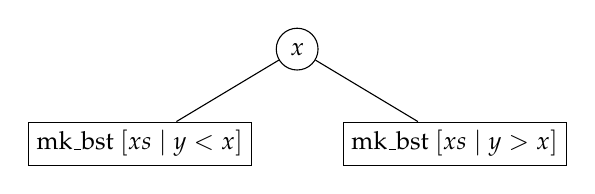
\begin{tikzpicture}[level distance = 1.2cm, sibling distance=4cm]
\small
\node[shape=circle,draw] {$x$}
  child {node[shape=rectangle,draw]{$\text{mk\_bst}\ [xs\mid y < x]$}}
  child {node[shape=rectangle,draw]{$\text{mk\_bst}\ [xs\mid y > x]$}};
\end{tikzpicture}
}\pause\\[0.5em]
Let us now add elements from a set $A$ in random order:
\vspace*{-0.5em}
\[\text{rbst}\ A := \textbf{do}\ \{\textit{xs} \leftarrow \text{rperm}\ A;\ \textbf{return}\ (\text{mk\_bst}\ \textit{xs})\}\]\pause
\vspace*{-1.5em}
\begin{lemma}
\upshape
\vspace*{-1em}
\begin{tabbing}
\hskip2em $\text{rbst}\ A = \textbf{do}\ $\= $x \leftarrow \text{uniform}\ A$\hspace*{5.1cm}\\
\> $l \leftarrow \text{rbst}\ \{y\in A\mid y < x\}$\\
\> $r \leftarrow \text{rbst}\ \{y\in A\mid y > x\}$\\[1mm]
\> $\textbf{return}$\ \bigg(\resizebox{1.7cm}{!}{\raisebox{-5mm}{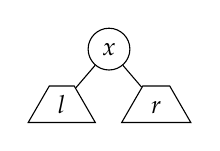
\begin{tikzpicture}[level distance=7mm, sibling distance=12mm]\small\node[shape=circle,draw] {$x$} 
child {node[draw, trapezium, trapezium angle=60, text height=1.5mm]{\raisebox{-1mm}{$l$}}} child {node[draw, trapezium, trapezium angle=60, text height=1.5mm]{\raisebox{-1mm}{$r$}}};\end{tikzpicture}}}\bigg)
\end{tabbing}
\vspace*{-1em}
\end{lemma}
\end{frame}

\begin{frame}
The height is somewhat more difficult: [CLRS]\pause
\[\text{eheight\_rbst}\ A := \textbf{do}\ \{t \leftarrow \text{rbst}\ A; \textbf{return}\ 2^{\text{height}\ t - 1}\}\]\pause
\vspace*{-1.5em}
\begin{theorem}\upshape
\vspace*{-0.4em}
\begin{itemize}
\item 
\begin{tabbing}
$\text{eheight\_rbst}\ A = \textbf{do}\ $\= $x \leftarrow \text{uniform}\ A$\\
\> $l \leftarrow \text{eheight\_rbst}\ \{y\in A\mid y < x\}$\\
\> $r \leftarrow \text{eheight\_rbst}\ \{y\in A\mid y > x\}$\\
\> $\textbf{return}\ (2 \cdot \text{max}\ l\ r)$
\end{tabbing}
\pause
\item
$\expectation[\text{eheight\_rbst}(n)] \leq \frac{4}{n}\cdot \sum_{i=0}^{n-1} \expectation[\text{eheight\_rbst}(i)]$\pause\\[3mm]
\item
$\expectation[\text{eheight\_rbst}(n)] \leq \frac{1}{4} {{n + 3} \choose 3}$\\[2mm]\pause% = \frac{1}{24}(n+1)(n+2)(n+3)$\\[2mm]
\item
$\expectation[\text{height}(\text{rbst}(n))] \leq \log_2 {{n + 3} \choose 3} - 1\pause \sim 3 \log_2 n$\pause
\end{itemize}
\end{theorem}
The actual behaviour is $\approx 2.988 \log_2 n$ [Reed 2003].

\end{frame}
\begin{frame}
\begin{center}
\huge\high{Vector Spaces}
\end{center}
\end{frame}

\begin{frame}
A \emph{vector space} $V$ over a field $K$ is an Abelian group (like $(\mathbb{R},+,0)$) together with a \emph{scale} operator $\odot:K\times V \to V$ such that for 
%to-do
Examples:
\begin{itemize}%to-do
\item If $K$ is a field, then $K/K$ is a field extension\pause
%problem for a formalisation: K is often identified with its carrier set
\item $\mathbb{R}/\mathbb{Q}$ is a field extension
\end{itemize}
\end{frame}

\begin{frame}
\begin{center}
\huge\high{Field Extensions}
\end{center}
\end{frame}

\begin{frame}
A \emph{field} is a nontrivial commutative ring where every nonzero element has a multiplicative inverse.

A \emph{field extension} ($L/K$) is a field $L$ where $K$ is a subset of $L$'s carrier set and $K$ together with $\otimes,1,\oplus,0$ is again a field.
%to-do: use records?
\begin{itemize}
\item If $K$ is a field, then $K/K$ is a field extension\pause
%problem for a formalisation: K is often identified with its carrier set
\item $\mathbb{R}/\mathbb{Q}$ is a field extension
\end{itemize}
\end{frame}

\begin{frame}
\high{If priorities are distinct, the shape of a treap is thus uniquely defined by its entries.}\pause\\[1em]
\begin{tabbing}
$\Longrightarrow$\ \= Insert list of elements into a treap in \emph{any} order ${\simeq}$\\
\> Insert elements into a BST by increasing priority
\end{tabbing}\pause
\high{Idea:} Choose priority randomly from $[0;1] \subseteq \mathbb{R}$ upon insertion\\\pause
$\Longrightarrow$\ Treap behaves like a random BST\\\pause
\begin{center}
\high{Randomised Treap}
\end{center}
\end{frame}

\begin{frame}{Definition of some operations on treaps}
\begin{tabbing}
$\text{ins} :: (\alpha \times \mathbb{R}) \Rightarrow (\alpha, \mathbb{R})\ \text{treap} \Rightarrow (\alpha, \mathbb{R})\ \text{treap}$\\[4mm]\pause
$\text{rins} :: \alpha \Rightarrow (\alpha, \mathbb{R})\ \text{treap} \Rightarrow (\alpha, \mathbb{R})\ \text{treap}$\\[0.5mm]
$\text{rins}\ x\ t = \textbf{do}\ \{p \leftarrow \mathcal U;\ \textbf{return}\ (\text{ins}\ (x, p)\ t)\}$\\[4mm]\pause
$\text{rinss} :: \alpha\ \text{list} \Rightarrow (\alpha, \mathbb{R})\ \text{treap} \Rightarrow (\alpha, \mathbb{R})\ \text{treap}$\\[0.5mm]
$\text{rinss}\ \listnil\ t = \textbf{return}\ t$\\
$\text{rinss}\ ([x]\listapp \textit{xs})\ t = \textbf{do}\ \{t' \leftarrow \text{rins}\ x\ t;\ \text{rinss}\ \textit{xs}\ t'\}$
\end{tabbing}
\end{frame}

\begin{frame}{Proof of the main result on treaps:}
\begin{center}
\parbox{0cm}{
\small
\begin{tabbing}
$\text{rinss}\ \textit{xs} $\=${}= \textbf{do}\ \{p \leftarrow \mathcal U^{\textit{xs}}; \textbf{return}\ \text{treap\_of}\ [(x, p(x))\mid x\leftarrow \textit{xs}]\}$\\[2mm]\pause
\>${}\hskip-1.8mm\stackrel{\text{\tiny project}}\simeq \hskip-1.8mm\textbf{do}\ \{p \leftarrow \mathcal U^{\textit{xs}}; \textbf{return}\ \text{mk\_bst}\ (\text{sort\_key}\ p\ \textit{xs})\}$\\[2mm]\pause
\>${}= \textbf{do}\ \{$\=$R \leftarrow \text{rel\_from\_prios}\ \mathcal U^{\textit{xs}};$\\\>\> $\textbf{return}\ \text{mk\_bst}\ (\text{sort\_rel}\ R\ \textit{xs})\}$\\[2mm]\pause
\>${}= \textbf{do}\ \{$\=$R \leftarrow \text{uniform}\ (\text{linorder\_on}\ R);$\\\>\> $\textbf{return}\ \text{mk\_bst}\ (\text{sort\_rel}\ R\ \textit{xs})\}$\\[2mm]\pause
\>${}= \textbf{do}\ \{$\=$\textit{xs'} \leftarrow \text{rperm}\ \textit{xs};\ \textbf{return}\ \text{mk\_bst}\ \textit{xs'}\}$\\[2mm]\pause
\>${}= \text{random\_bst}\ \textit{xs}$
\end{tabbing}}\\[-2em]\pause
\mbox{}\hspace*{\fill}$\square$\hspace*{1em}
\end{center}
\end{frame}

\begin{frame}{Measures}
\bad{Problem:} Random treaps are a \emph{continuous} distribution\\ $\Longrightarrow$ cannot use PMFs\\[1em]\pause

Instead we have to use general measures $(\Omega, \Sigma, \mu)$\\[1em]\pause

\bad{But what does a suitable $\Sigma$-algebra for trees look like?}\pause
\begin{itemize}
\item Functor $\mathcal T$ that maps a $\Sigma$-algebra over a set $A$ to a $\Sigma$-algebra of trees with elements from $A$\pause
\item The \enquote{Node} constructor is a measurable function from $\mathcal T(M)\otimes M\otimes \mathcal T(M)$ to $\mathcal T(M)$\pause
\item Other tree operations (projections, primitive recursion) are similarly measurable
\end{itemize}
\end{frame}

\tikzstyle{bag} = [align=center]
\begin{frame}
\begin{center}
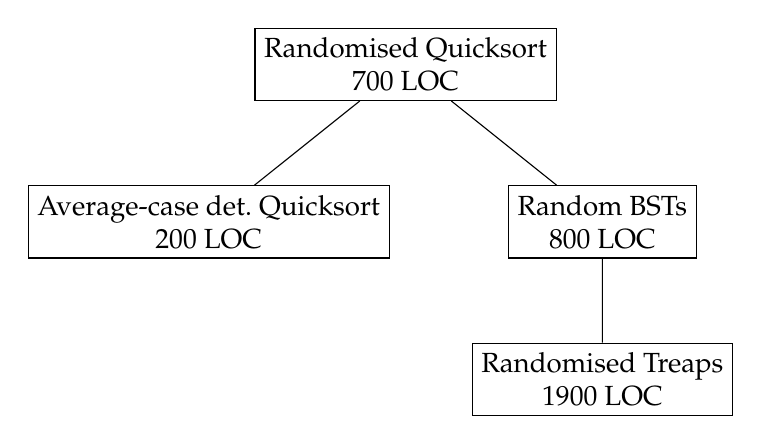
\begin{tikzpicture}[level distance = 2cm, sibling distance=5cm]
\node[shape=rectangle,draw,align=center] {Randomised Quicksort\\ 700 LOC}
  child { node[shape=rectangle,draw,align=center] {Average-case det.\ Quicksort\\ 200 LOC} }
  child { node[shape=rectangle,draw,align=center] {Random BSTs\\ 800 LOC} 
    child { node[shape=rectangle,draw,align=center] {Randomised Treaps\\ 1900 LOC} }
  };
\end{tikzpicture}\hspace*{2em}
\end{center}
\end{frame}

\begin{frame}{Bonus: Executability}
\small
\textbf{value}\ random\_bst\ $\{1, 2, 3 :: \text{int}\}$\pause\\[-1em]
\hskip1em \parbox{0cm}{
\begin{tabbing}
pmf\_of\_alist\\
\hskip5mm $[$\=$(\langle\langle\langle\langle\rangle, 1, \langle\rangle\rangle, 2, \langle\rangle\rangle, 3, \langle\rangle\rangle, 1 / 6),$\\
   \>$(\langle\langle\langle\rangle, 1, \langle\langle\rangle, 2, \langle\rangle\rangle\rangle, 3, \langle\rangle\rangle, 1 / 6),$\\
   \>$(\langle\langle\rangle, 1, \langle\langle\langle\rangle, 2, \langle\rangle\rangle, 3, \langle\rangle\rangle\rangle, 1 / 6),$\\
   \>$(\langle\langle\langle\rangle, 1, \langle\rangle\rangle, 2, \langle\langle\rangle, 3, \langle\rangle\rangle\rangle, 1 / 3),$\\
   \>$(\langle\langle\rangle, 1, \langle\langle\rangle, 2, \langle\langle\rangle, 3, \langle\rangle\rangle\rangle\rangle, 1 / 6)]$\\
   \>\hskip5mm int\ tree\ pmf
\end{tabbing}}
\pause\\
\textbf{value}\ measure\_pmf.expectation\ $($random\_bst\ $\{1..6::\text{int}\})$\ height\pause\\[2mm]
\hskip1.2em 65 / 15 :: real
\end{frame}

\begin{frame}{Conclusion}
\begin{itemize}
\item Formalisation of textbook randomised algorithms/data structures is feasible with Isabelle\pause
\item PMF proofs are nice, high-level, and readable\pause
\item Measure proofs can get ugly due to measurability issues\pause
\end{itemize}
Interesting related topics:\pause
\begin{itemize}
\item Tail bounds [Tassarotti \& Harper 2018]\pause
\item Treaps can also use discrete distributions\pause
\item Randomised BSTs [Martinez \& Roura 1997]\pause
\item Skip Lists (already done, [Haslbeck \& E.\ 2018])
\end{itemize}
\end{frame}


\end{document}
